%%%%%%%%%%%%%%%%%%%%%%%%%%%%%%%%%%%%%%%%%%%%%%%%%%%
%% P3: Phenomenology of Particle Physics                         
%%
%% Author:  André Rubbia                   		 
%%
%% Figure 18.8 Graphical plots of the different terms in the QCD matrix elements as a function of $t/s$. 
%%
%% This work is licensed under the Creative Commons Attribution 4.0 International License. 
%% To view a copy of this license, visit http://creativecommons.org/licenses/by/4.0/ or 
%% send a letter to Creative Commons, PO Box 1866, Mountain View, CA 94042, USA.
%%
%%%%%%%%%%%%%%%%%%%%%%%%%%%%%%%%%%%%%%%%%%%%%%%%%%%

\documentclass[a4paper,10pt]{article}

\usepackage[T1]{fontenc}
\usepackage[utf8]{inputenc}
\usepackage{lmodern}
\usepackage[labelfont=bf]{caption}
\usepackage{upgreek}
\usepackage{braket}

\usepackage{tikz}
\usepackage{pgfplots}
\pgfplotsset{compat=1.17}
\usepgfplotslibrary{ternary}
\usepgfplotslibrary{fillbetween}
\usepgfplotslibrary{external}

\def\d{\mathrm{d}}

\begin{document}

%%%%%%%%%%%%%%%   FIGURE  %%%%%%%%%%%%%%%%%%%%%%%%%%%%%%
\begin{figure}[htbp]
\begin{center}
\pgfplotsset{every axis/.append
    style={
%    font=\large,
    line width=1pt,
    tick style={line width=0.8pt}}}
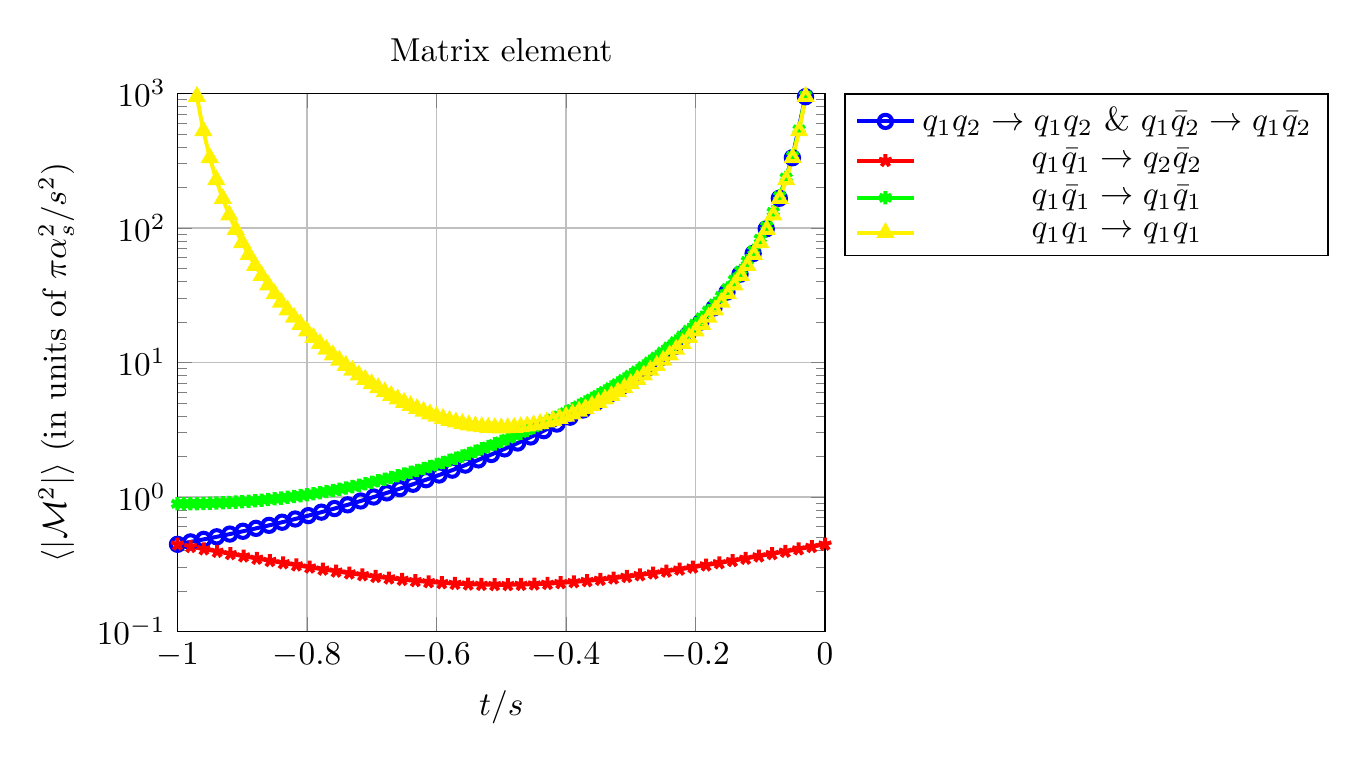
\begin{tikzpicture}[scale=1.2]
    \begin{semilogyaxis}[
        title=Matrix element,
        xlabel={$t/s$},
        ylabel={$\braket{\vert{\cal M}^2\vert}$ (in units of $\pi\alpha_s^2/s^2$)},
        xmin=-1, xmax=0,
        ymin = 1e-1, ymax=1000,
        minor y tick num=1,
        grid = major,
        legend entries={
        $q_1q_2\rightarrow q_1q_2$ \& $q_1\bar q_2\rightarrow q_1\bar q_2$,
        $q_1\bar q_1\rightarrow q_2\bar q_2$,
        $q_1 \bar q_1\rightarrow q_1 \bar q_1$,
       $q_1 q_1\rightarrow q_1 q_1$,
       $q \bar q\rightarrow gg$,
       $q g \rightarrow qg$,
       $gg \rightarrow q\bar q$,
       $gg \rightarrow gg$
        },
        legend style={legend pos = outer north east}
    ]
%  q1q2 → q1 q2, q1 bar q2 -> q1 bar q2
        \addplot [blue,very thick,samples=50,domain=-1:-0.01, mark=o] {(4/9)*((1/x)^2+((1+x)/x)^2)};
 %  q1 bar q1 → q2 bar q2
       \addplot [red,very thick, samples=50,domain=-1:0, mark=star] {(4/9)*(x^2+(1+x)^2)};

%  q1 bar q1 -> q1 bar q1
        \addplot [green,very thick, mark=asterisk]
	 coordinates {
	 (-1,0.888889)(-0.99,0.889188)(-0.98,0.890098)(-0.97,0.891639)(-0.96,0.89383)(-0.95,0.896692)(-0.94,0.900249)(-0.93,0.904525)(-0.92,0.909544)(-0.91,0.915333)(-0.9,0.92192)(-0.89,0.929336)(-0.88,0.937612)(-0.87,0.946781)(-0.86,0.956879)(-0.85,0.967943)(-0.84,0.980014)(-0.83,0.993135)(-0.82,1.00735)(-0.81,1.02271)(-0.8,1.03926)(-0.79,1.05706)(-0.78,1.07617)(-0.77,1.09664)(-0.76,1.11856)(-0.75,1.14198)(-0.74,1.16698)(-0.73,1.19364)(-0.72,1.22206)(-0.71,1.25233)(-0.7,1.28454)(-0.69,1.3188)(-0.68,1.35523)(-0.67,1.39396)(-0.66,1.43513)(-0.65,1.47886)(-0.64,1.52534)(-0.63,1.57472)(-0.62,1.62719)(-0.61,1.68295)(-0.6,1.74222)(-0.59,1.80524)(-0.58,1.87226)(-0.57,1.94357)(-0.56,2.01947)(-0.55,2.10029)(-0.54,2.18642)(-0.53,2.27824)(-0.52,2.37621)(-0.51,2.48082)(-0.5,2.59259)(-0.49,2.71214)(-0.48,2.84011)(-0.47,2.97724)(-0.46,3.12435)(-0.45,3.28233)(-0.44,3.45221)(-0.43,3.63512)(-0.42,3.83233)(-0.41,4.04527)(-0.4,4.27556)(-0.39,4.52503)(-0.38,4.79575)(-0.37,5.0901)(-0.36,5.41078)(-0.35,5.76089)(-0.34,6.144)(-0.33,6.56424)(-0.32,7.02639)(-0.31,7.53605)(-0.3,8.09975)(-0.29,8.72521)(-0.28,9.42153)(-0.27,10.1996)(-0.26,11.0724)(-0.25,12.0556)(-0.24,13.1682)(-0.23,14.4337)(-0.22,15.8808)(-0.21,17.5454)(-0.2,19.4726)(-0.19,21.7198)(-0.18,24.3611)(-0.17,27.4928)(-0.16,31.2428)(-0.15,35.783)(-0.14,41.3494)(-0.13,48.2729)(-0.12,57.0281)(-0.11,68.3166)(-0.1,83.2089)(-0.09,103.405)(-0.08,131.736)(-0.07,173.199)
	 (-0.06,237.301)(-0.05,343.973)(-0.04,541.015)(-0.03,968.181)(-0.02,2192.88)(-0.01,8829.92)
	 };

	 %  q1 q1 -> q1 q1
        \addplot [yellow,very thick, mark=triangle]
	 coordinates {
	(-0.99,8770.97)(-0.98,2163.57)(-0.97,948.76)(-0.96,526.545)(-0.95,332.478)(-0.94,227.795)(-0.93,165.117)
(-0.92,124.725)(-0.91,97.2305)(-0.9,77.7064)(-0.89,63.3669)(-0.88,52.5418)(-0.87,44.1812)
(-0.86,37.5985)(-0.85,32.3298)(-0.84,28.0525)(-0.83,24.537)(-0.82,21.616)(-0.81,19.1656)(-0.8,17.0926)(-0.79,15.3254)(-0.78,13.8087)(-0.77,12.4991)(-0.76,11.3622)(-0.75,10.3704)(-0.74,9.50137)(-0.73,8.73706)(-0.72,8.06254)(-0.71,7.46552)(-0.7,6.93575)(-0.69,6.4647)(-0.68,6.04516)(-0.67,5.67107)(-0.66,5.33727)(-0.65,5.0394)(-0.64,4.77371)(-0.63,4.537)(-0.62,4.32654)(-0.61,4.13998)(-0.6,3.97531)(-0.59,3.83081)(-0.58,3.70501)(-0.57,3.59666)(-0.56,3.50472)(-0.55,3.42831)(-0.54,3.36673)(-0.53,3.31939)(-0.52,3.28589)(-0.51,3.2659)(-0.5,3.25926)(-0.49,3.2659)(-0.48,3.28589)(-0.47,3.31939)(-0.46,3.36673)(-0.45,3.42831)(-0.44,3.50472)(-0.43,3.59666)(-0.42,3.70501)(-0.41,3.83081)(-0.4,3.97531)(-0.39,4.13998)(-0.38,4.32654)(-0.37,4.537)(-0.36,4.77371)(-0.35,5.0394)(-0.34,5.33727)(-0.33,5.67107)(-0.32,6.04516)(-0.31,6.4647)(-0.3,6.93575)(-0.29,7.46552)(-0.28,8.06254)(-0.27,8.73706)(-0.26,9.50137)(-0.25,10.3704)(-0.24,11.3622)(-0.23,12.4991)(-0.22,13.8087)(-0.21,15.3254)(-0.2,17.0926)(-0.19,19.1656)(-0.18,21.616)(-0.17,24.537)(-0.16,28.0525)(-0.15,32.3298)(-0.14,37.5985)(-0.13,44.1812)(-0.12,52.5418)(-0.11,63.3669)(-0.1,77.7064)(-0.09,97.2305)(-0.08,124.725)(-0.07,165.117)
(-0.06,227.795)(-0.05,332.478)(-0.04,526.545)(-0.03,948.76)(-0.02,2163.57)(-0.01,8770.97)
};

   \end{semilogyaxis}
\end{tikzpicture}%

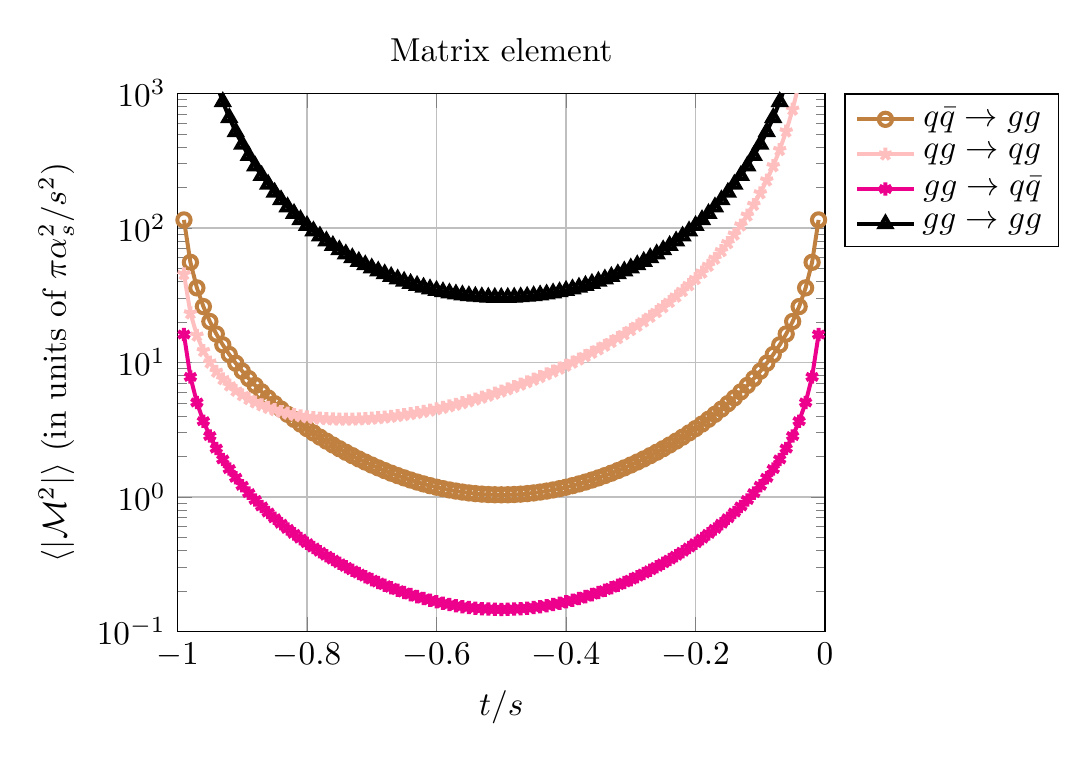
\begin{tikzpicture}[scale=1.2]
       \begin{semilogyaxis}[
        title=Matrix element,
        xlabel={$t/s$},
        ylabel={$\braket{\vert{\cal M}^2\vert}$ (in units of $\pi\alpha_s^2/s^2$)},
        xmin=-1, xmax=0,
        ymin = 1e-1, ymax=1000,
        minor y tick num=1,
        grid = major,
        legend entries={
       $q \bar q\rightarrow gg$,
       $q g \rightarrow qg$,
       $gg \rightarrow q\bar q$,
       $gg \rightarrow gg$
        },
        legend style={legend pos = outer north east}
    ]

	 %  q bar q → g g
        \addplot [brown,very thick, mark=o]
	 coordinates {
(-0.99,114.731)(-0.98,55.5361)(-0.97,35.8462)(-0.96,26.032)(-0.95,20.1676)(-0.94,16.2777)(-0.93,13.5158)(-0.92,11.4586)(-0.91,9.87089)(-0.9,8.61169)(-0.89,7.59118)(-0.88,6.74951)(-0.87,6.04525)(-0.86,5.44883)(-0.85,4.93853)(-0.84,4.49811)(-0.83,4.11511)(-0.82,3.77987)(-0.81,3.48477)(-0.8,3.2237)(-0.79,2.99174)(-0.78,2.78484)(-0.77,2.59968)(-0.76,2.43349)(-0.75,2.28395)(-0.74,2.1491)(-0.73,2.02728)(-0.72,1.91706)(-0.71,1.81722)(-0.7,1.7267)(-0.69,1.6446)(-0.68,1.57012)(-0.67,1.50257)(-0.66,1.44134)(-0.65,1.3859)(-0.64,1.3358)(-0.63,1.29061)(-0.62,1.24999)(-0.61,1.21363)(-0.6,1.18123)(-0.59,1.15258)(-0.58,1.12746)(-0.57,1.10568)(-0.56,1.0871)(-0.55,1.07159)(-0.54,1.05904)(-0.53,1.04937)(-0.52,1.0425)(-0.51,1.0384)(-0.5,1.03704)(-0.49,1.0384)(-0.48,1.0425)(-0.47,1.04937)(-0.46,1.05904)(-0.45,1.07159)(-0.44,1.0871)(-0.43,1.10568)(-0.42,1.12746)(-0.41,1.15258)(-0.4,1.18123)(-0.39,1.21363)(-0.38,1.24999)(-0.37,1.29061)(-0.36,1.3358)(-0.35,1.3859)(-0.34,1.44134)(-0.33,1.50257)(-0.32,1.57012)(-0.31,1.6446)(-0.3,1.7267)(-0.29,1.81722)(-0.28,1.91706)(-0.27,2.02728)(-0.26,2.1491)(-0.25,2.28395)(-0.24,2.43349)(-0.23,2.59968)(-0.22,2.78484)(-0.21,2.99174)(-0.2,3.2237)(-0.19,3.48477)(-0.18,3.77987)(-0.17,4.11511)(-0.16,4.49811)(-0.15,4.93853)(-0.14,5.44883)(-0.13,6.04525)(-0.12,6.74951)(-0.11,7.59118)(-0.1,8.61169)(-0.09,9.87089)(-0.08,11.4586)(-0.07,13.5158)(-0.06,16.2777)(-0.05,20.1676)(-0.04,26.032)(-0.03,35.8462)(-0.02,55.5361)(-0.01,114.731)
};

	 %  q g - > q g
        \addplot [pink,very thick, mark=star]
	 coordinates {
(-0.99,45.4693)(-0.98,23.2728)(-0.97,15.8919)(-0.96,12.2157)(-0.95,10.0219)(-0.94,8.56988)(-0.93,7.54219)(-0.92,6.78015)(-0.91,6.19564)(-0.9,5.7358)(-0.89,5.36704)(-0.88,5.06695)(-0.87,4.82009)(-0.86,4.61541)(-0.85,4.44485)(-0.84,4.3024)(-0.83,4.18348)(-0.82,4.08453)(-0.81,4.00281)(-0.8,3.93611)(-0.79,3.8827)(-0.78,3.84119)(-0.77,3.81044)(-0.76,3.78954)(-0.75,3.77778)(-0.74,3.77456)(-0.73,3.77941)(-0.72,3.79199)(-0.71,3.81202)(-0.7,3.8393)(-0.69,3.87372)(-0.68,3.91519)(-0.67,3.96373)(-0.66,4.01937)(-0.65,4.0822)(-0.64,4.15238)(-0.63,4.2301)(-0.62,4.31559)(-0.61,4.40915)(-0.6,4.51111)(-0.59,4.62188)(-0.58,4.7419)(-0.57,4.87167)(-0.56,5.01178)(-0.55,5.16286)(-0.54,5.32563)(-0.53,5.5009)(-0.52,5.68956)(-0.51,5.89259)(-0.5,6.11111)(-0.49,6.34636)(-0.48,6.5997)(-0.47,6.87268)(-0.46,7.16702)(-0.45,7.48462)(-0.44,7.82766)(-0.43,8.19856)(-0.42,8.60003)(-0.41,9.03515)(-0.4,9.50741)(-0.39,10.0207)(-0.38,10.5797)(-0.37,11.1893)(-0.36,11.8554)(-0.35,12.5849)(-0.34,13.3854)(-0.33,14.266)(-0.32,15.2371)(-0.31,16.3108)(-0.3,17.5016)(-0.29,18.8262)(-0.28,20.3046)(-0.27,21.9607)(-0.26,23.823)(-0.25,25.9259)(-0.24,28.3115)(-0.23,31.031)(-0.22,34.1479)(-0.21,37.7414)(-0.2,41.9111)(-0.19,46.784)(-0.18,52.5237)(-0.17,59.3438)(-0.16,67.5274)(-0.15,77.4562)(-0.14,89.6541)(-0.13,104.856)(-0.12,124.118)(-0.11,149.002)(-0.1,181.894)(-0.09,226.584)(-0.08,289.392)(-0.07,381.483)(-0.06,524.113)(-0.05,761.89)(-0.04,1201.89)(-0.03,2157.44)(-0.02,4901.89)(-0.01,19801.9)
};

	 %  g g - > q bar q
        \addplot [magenta,very thick, mark=asterisk]
	 coordinates {
(-0.99,16.1341)(-0.98,7.80977)(-0.97,5.04087)(-0.96,3.66074)(-0.95,2.83606)(-0.94,2.28905)(-0.93,1.90066)(-0.92,1.61136)(-0.91,1.38809)(-0.9,1.21102)(-0.89,1.06751)(-0.88,0.949149)(-0.87,0.850114)(-0.86,0.766241)(-0.85,0.694481)(-0.84,0.632546)(-0.83,0.578687)(-0.82,0.531545)(-0.81,0.490046)(-0.8,0.453333)(-0.79,0.420713)(-0.78,0.391618)(-0.77,0.36558)(-0.76,0.342209)(-0.75,0.321181)(-0.74,0.302218)(-0.73,0.285086)(-0.72,0.269586)(-0.71,0.255546)(-0.7,0.242817)(-0.69,0.231272)(-0.68,0.220798)(-0.67,0.211298)(-0.66,0.202688)(-0.65,0.194892)(-0.64,0.187846)(-0.63,0.181492)(-0.62,0.17578)(-0.61,0.170666)(-0.6,0.166111)(-0.59,0.162082)(-0.58,0.158548)(-0.57,0.155486)(-0.56,0.152874)(-0.55,0.150692)(-0.54,0.148927)(-0.53,0.147567)(-0.52,0.146602)(-0.51,0.146025)(-0.5,0.145833)(-0.49,0.146025)(-0.48,0.146602)(-0.47,0.147567)(-0.46,0.148927)(-0.45,0.150692)(-0.44,0.152874)(-0.43,0.155486)(-0.42,0.158548)(-0.41,0.162082)(-0.4,0.166111)(-0.39,0.170666)(-0.38,0.17578)(-0.37,0.181492)(-0.36,0.187846)(-0.35,0.194892)(-0.34,0.202688)(-0.33,0.211298)(-0.32,0.220798)(-0.31,0.231272)(-0.3,0.242817)(-0.29,0.255546)(-0.28,0.269586)(-0.27,0.285086)(-0.26,0.302218)(-0.25,0.321181)(-0.24,0.342209)(-0.23,0.36558)(-0.22,0.391618)(-0.21,0.420713)(-0.2,0.453333)(-0.19,0.490046)(-0.18,0.531545)(-0.17,0.578687)(-0.16,0.632546)(-0.15,0.694481)(-0.14,0.766241)(-0.13,0.850114)(-0.12,0.949149)(-0.11,1.06751)(-0.1,1.21102)(-0.09,1.38809)(-0.08,1.61136)(-0.07,1.90066)(-0.06,2.28905)(-0.05,2.83606)(-0.04,3.66074)(-0.03,5.04087)(-0.02,7.80977)(-0.01,16.1341)
};

	 %  g g - > gg
	 \addplot [black,very thick, mark=triangle]
	 coordinates {
(-0.99,44563.5)(-0.98,11038.5)(-0.97,4863.51)(-0.96,2713.52)(-0.95,1723.54)(-0.94,1188.55)(-0.93,867.653)(-0.92,660.469)(-0.91,519.176)(-0.9,418.651)(-0.89,344.676)(-0.88,288.722)(-0.87,245.421)(-0.86,211.259)(-0.85,183.861)(-0.84,161.572)(-0.83,143.214)(-0.82,127.929)(-0.81,115.08)(-0.8,104.186)(-0.79,94.8799)(-0.78,86.8757)(-0.77,79.9497)(-0.76,73.924)(-0.75,68.6562)(-0.74,64.0312)(-0.73,59.9548)(-0.72,56.3499)(-0.71,53.1527)(-0.7,50.3101)(-0.69,47.7776)(-0.68,45.5178)(-0.67,43.4991)(-0.66,41.6946)(-0.65,40.0816)(-0.64,38.6405)(-0.63,37.3546)(-0.62,36.2096)(-0.61,35.1933)(-0.6,34.295)(-0.59,33.5058)(-0.58,32.818)(-0.57,32.2251)(-0.56,31.7215)(-0.55,31.3027)(-0.54,30.9649)(-0.53,30.7052)(-0.52,30.5212)(-0.51,30.4115)(-0.5,30.375)(-0.49,30.4115)(-0.48,30.5212)(-0.47,30.7052)(-0.46,30.9649)(-0.45,31.3027)(-0.44,31.7215)(-0.43,32.2251)(-0.42,32.818)(-0.41,33.5058)(-0.4,34.295)(-0.39,35.1933)(-0.38,36.2096)(-0.37,37.3546)(-0.36,38.6405)(-0.35,40.0816)(-0.34,41.6946)(-0.33,43.4991)(-0.32,45.5178)(-0.31,47.7776)(-0.3,50.3101)(-0.29,53.1527)(-0.28,56.3499)(-0.27,59.9548)(-0.26,64.0312)(-0.25,68.6562)(-0.24,73.924)(-0.23,79.9497)(-0.22,86.8757)(-0.21,94.8799)(-0.2,104.186)(-0.19,115.08)(-0.18,127.929)(-0.17,143.214)(-0.16,161.572)(-0.15,183.861)(-0.14,211.259)(-0.13,245.421)(-0.12,288.722)(-0.11,344.676)(-0.1,418.651)(-0.09,519.176)(-0.08,660.469)(-0.07,867.653)(-0.06,1188.55)(-0.05,1723.54)(-0.04,2713.52)(-0.03,4863.51)(-0.02,11038.5)(-0.01,44563.5)
};

   \end{semilogyaxis}
\end{tikzpicture}%
\caption{Graphical plots of the different terms
in the matrix elements as a function of $t/s$. The $u$  variable is given by
$u/s=-(1+t/s)$.}
\end{center}
\end{figure}
%%%%%%%%%%%%%%%  END FIGURE  %%%%%%%%%%%%%%%%%%%%%%%%%%%%%%
%

\end{document}
